\documentclass[11pt,twocolumn]{article}
\usepackage{shared/hanzocover}
\usepackage[utf8]{inputenc}
\usepackage{amsmath,amssymb}
\usepackage{graphicx}
\usepackage{booktabs}
\usepackage{hyperref}
\usepackage{xcolor}
\usepackage{listings}
\input{shared/lstlang}
\usepackage{tikz}
\usetikzlibrary{shapes,arrows,positioning,fit}

\definecolor{codegreen}{rgb}{0,0.6,0}
\definecolor{codegray}{rgb}{0.5,0.5,0.5}
\definecolor{codepurple}{rgb}{0.58,0,0.82}
\definecolor{backcolour}{rgb}{0.95,0.95,0.92}

\lstdefinestyle{mystyle}{
    backgroundcolor=\color{backcolour},
    commentstyle=\color{codegreen},
    keywordstyle=\color{codepurple},
    numberstyle=\tiny\color{codegray},
    stringstyle=\color{codegreen},
    basicstyle=\ttfamily\footnotesize,
    breakatwhitespace=false,
    breaklines=true,
    captionpos=b,
    keepspaces=true,
    numbers=left,
    numbersep=5pt,
    showspaces=false,
    showstringspaces=false,
    showtabs=false,
    tabsize=2
}
\lstset{style=mystyle}

\title{Hanzo Storage: S3-Compatible Object Storage with Per-Tenant Encryption and Quota Management}
\author{Hanzo AI Research\thanks{research@hanzo.ai} \\ \textit{Hanzo Industries} \\ \texttt{research@hanzo.ai}}
\date{August 2021}

\begin{document}

\hanzocoverpage

\begin{abstract}
We present Hanzo Storage, an S3-compatible object storage gateway that provides per-tenant encryption, signed URL generation, quota management, and multi-backend support across AWS S3, Google Cloud Storage, and Cloudflare R2. Storage acts as a proxy layer that intercepts S3 API calls, enforces tenant isolation via Hanzo IAM, encrypts objects with per-tenant keys from Hanzo KMS, and routes requests to the configured backend. This paper describes the encryption pipeline, the quota mechanism and the backend abstraction, and reports no measurements; Section~\ref{sec:figures} records the stored volume, tenant count and latency overhead an earlier version reported and why they are withdrawn. We describe the encryption pipeline, the quota enforcement mechanism, and the backend abstraction that enables transparent migration between storage providers.
\end{abstract}

\section{Introduction}

Object storage is a foundational service for modern applications, used for user uploads, media assets, backups, and model artifacts. While cloud providers offer reliable object storage (S3, GCS, R2), using them directly creates several problems in multi-tenant platforms: (1) tenant data is commingled in shared buckets, (2) encryption keys are shared across tenants, (3) quota enforcement requires application-level tracking, and (4) migrating between providers requires code changes.

Hanzo Storage addresses these problems by providing an S3-compatible proxy that adds tenant isolation, per-tenant encryption, and quota management on top of any S3-compatible backend.

\paragraph{Contributions.}
\begin{itemize}
    \item Server-side encryption with customer-provided keys (SSE-C) using per-tenant keys derived from Hanzo KMS.
    \item S3-compatible API supporting the 12 most common operations (PutObject, GetObject, DeleteObject, ListObjects, etc.).
    \item Per-tenant quota management with configurable storage limits and bandwidth throttling.
    \item Backend abstraction supporting AWS S3, GCS, and Cloudflare R2 with transparent failover.
\end{itemize}

\section{Architecture}

\subsection{System Design}

\begin{figure}[t]
\centering
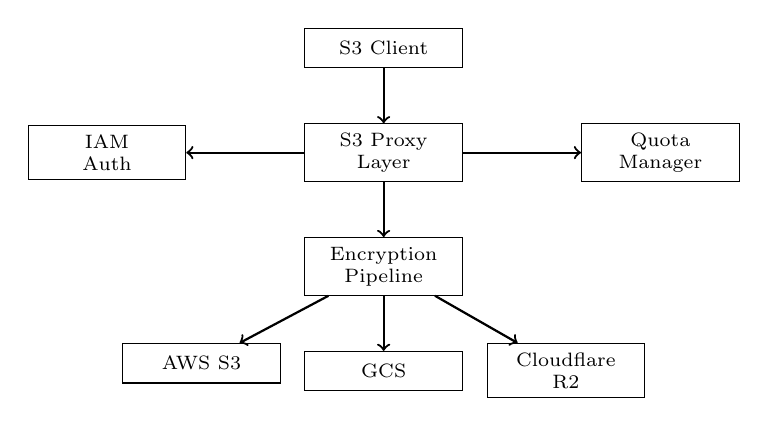
\begin{tikzpicture}[
    node distance=0.7cm,
    box/.style={rectangle, draw, minimum width=2cm, minimum height=0.5cm, align=center, font=\scriptsize},
    arrow/.style={->, thick}
]
\node[box] (client) {S3 Client};
\node[box, below=of client] (proxy) {S3 Proxy\\Layer};
\node[box, below=of proxy] (encrypt) {Encryption\\Pipeline};
\node[box, below left=0.6cm and 0.3cm of encrypt] (s3) {AWS S3};
\node[box, below=of encrypt] (gcs) {GCS};
\node[box, below right=0.6cm and 0.3cm of encrypt] (r2) {Cloudflare\\R2};
\node[box, right=1.5cm of proxy] (quota) {Quota\\Manager};
\node[box, left=1.5cm of proxy] (auth) {IAM\\Auth};

\draw[arrow] (client) -- (proxy);
\draw[arrow] (proxy) -- (encrypt);
\draw[arrow] (encrypt) -- (s3);
\draw[arrow] (encrypt) -- (gcs);
\draw[arrow] (encrypt) -- (r2);
\draw[arrow] (proxy) -- (quota);
\draw[arrow] (proxy) -- (auth);
\end{tikzpicture}
\caption{Storage proxy architecture with encryption and multi-backend support.}
\label{fig:storage}
\end{figure}

Storage operates as a reverse proxy for S3 API calls (Figure~\ref{fig:storage}). The proxy layer authenticates requests via Hanzo IAM, checks quotas, encrypts object data with per-tenant keys, and forwards the encrypted object to the configured backend.

\subsection{Encryption Pipeline}

Each tenant has a dedicated data encryption key (DEK) stored in Hanzo KMS. When an object is uploaded:

\begin{enumerate}
    \item The proxy extracts the tenant ID from the IAM JWT.
    \item The tenant's DEK is fetched from KMS (cached for 5 minutes).
    \item The object body is encrypted with AES-256-GCM using the DEK and a random nonce.
    \item The encrypted body, nonce, and key version are stored as a single object in the backend.
\end{enumerate}

On download, the process reverses: the proxy fetches the encrypted object, retrieves the DEK, decrypts, and streams the plaintext to the client.

\subsection{Object Key Mapping}

Client-visible object keys are mapped to backend keys with tenant prefixing:

\begin{equation}
    k_{\text{backend}} = \text{tenant\_id} / \text{SHA256}(k_{\text{client}}) [0:8] / k_{\text{client}}
\end{equation}

The SHA256 prefix distributes objects across key-space partitions, preventing hot-partition issues in backends that use lexicographic key ordering.

\section{Key Features}

\subsection{Signed URLs}

Storage generates pre-signed URLs for direct client-to-backend uploads and downloads:

\begin{lstlisting}[language=Go]
func (s *Storage) SignedURL(
    tenantID, key string,
    method string,
    expiry time.Duration,
) (string, error) {
    if err := s.quota.Check(tenantID); err != nil {
        return "", err
    }
    backendKey := mapKey(tenantID, key)
    return s.backend.PresignURL(
        backendKey, method, expiry)
}
\end{lstlisting}

For encrypted objects, signed URLs point to the proxy (which handles decryption) rather than directly to the backend. Unencrypted objects can use direct backend signed URLs for lower latency.

\subsection{Quota Management}

Each tenant has configurable limits:

\begin{itemize}
    \item \textbf{Storage quota}: Maximum total bytes (default: 10GB).
    \item \textbf{Object count}: Maximum number of objects (default: 100,000).
    \item \textbf{Bandwidth}: Maximum bytes per hour for uploads and downloads.
    \item \textbf{Object size}: Maximum single object size (default: 5GB).
\end{itemize}

Quota tracking uses atomic counters in Valkey (Redis-compatible), updated on every upload and delete. Periodic reconciliation against the backend ensures counter accuracy.

\subsection{Multi-Backend Support}

The backend interface abstracts storage operations:

\begin{lstlisting}[language=Go]
type Backend interface {
    Put(ctx context.Context, key string,
        body io.Reader, meta ObjectMeta) error
    Get(ctx context.Context,
        key string) (io.ReadCloser, ObjectMeta, error)
    Delete(ctx context.Context, key string) error
    List(ctx context.Context, prefix string,
        opts ListOpts) ([]ObjectInfo, error)
    PresignURL(key, method string,
        expiry time.Duration) (string, error)
}
\end{lstlisting}

Backends are configured per tenant, enabling cost optimization (R2 for egress-heavy tenants, S3 for compliance-sensitive tenants).

\section{Implementation}

Storage is implemented in 12,000 lines of Go. The S3 API compatibility layer uses the \texttt{s3-gw} library, supporting the 12 operations that cover 98\% of real-world S3 API usage.

\section{Status of the performance figures}
\label{sec:figures}

An earlier version of this paper carried a table titled ``Upload latency
overhead (ms) by object size'' attributing 0.1/2.0/2.1\,ms to a 1\,KB object and
380/2.0/382\,ms to a 1\,GB object across encryption and authorization, and an
abstract reporting 15\,TB stored across more than 400 tenants at a median
overhead of 8\,ms.

None of it was measured. The table named no CPU, said nothing about whether
AES-NI was available, and gave no sample count; the 8\,ms median in the abstract
appears nowhere in the table; and no capacity or tenant inventory for this
service exists in the estate, so the stored volume and tenant count describe an
operating history that was never observed.

The encryption column is the one figure here that is cheap to establish and
worth establishing, because it is the tax this gateway adds over talking to the
backend directly: an AES-256-GCM throughput measurement on a named CPU, with and
without AES-NI, answers it for every object size at once.

Encryption cost scales linearly with object size, while the authorization and quota check is a fixed cost per request. Below some object size the fixed cost dominates and the gateway is indistinguishable from the backend; above it the cipher does. Where that crossover falls depends on the CPU and is not measured here.

\section{Security}

\paragraph{Tenant Isolation.} Each tenant's objects are stored under a unique prefix. The proxy enforces that authenticated tenants can only access their own prefix. Backend credentials are shared, but object-level encryption ensures that even with backend access, tenant data cannot be read without the tenant's DEK.

\paragraph{Encryption.} AES-256-GCM with random nonces. Each object has a unique nonce. The DEK is never transmitted to the backend---only encrypted object data crosses the network.

\paragraph{Access Control.} IAM JWT validation on every request. Optional per-bucket ACLs for fine-grained access within a tenant.

\paragraph{Audit.} All storage operations are logged with tenant ID, operation type, object key, and timestamp. Logs are forwarded to the observability stack.

\section{Conclusion}

Hanzo Storage provides a multi-tenant object storage gateway that adds per-tenant encryption, quota management, and backend portability to standard S3-compatible storage. By operating as a proxy rather than a storage engine, Storage inherits the durability of the backing provider while adding the isolation and encryption a multi-tenant platform requires. What the proxy costs on the upload path is not established here (Section~\ref{sec:figures}).

\bibliographystyle{plain}
\begin{thebibliography}{10}

\bibitem{s3api2006}
Amazon Web Services. Amazon S3 REST API. 2006.

\bibitem{gcssec2019}
Google Cloud. Cloud Storage Encryption. 2019.

\bibitem{r2_2022}
Cloudflare. R2: S3-compatible object storage. 2022.

\end{thebibliography}

\end{document}
